\begin{frame}{Reconocimiento de Actividades}

\centering\resizebox{0.70\textwidth}{!}{%
\noindent\begin{minipage}[t][1\totalheight][b]{1\columnwidth}%
\begin{algorithmic}[1]
    \Require Conjunto de tiempos de subscripci�n de clientes $S$
	\Procedure{Reconocimiento}{$ S $}
		\alertline<1> \If {$S \textit{ est� vac�o } $}
 			\State\textit{Terminar}
		\EndIf 
		\alertline<2> \State $t_w \leftarrow 10$ 
        \Comment{Ventana de tiempo est�ndar de reconocimiento}
		\alertline<3> \State $t_{min} \leftarrow \min_{\forall s \in S} s$
		\alertline<4> \State Esperar $t_{min} - t_w$ segundos 
		\alertline<5> \State $ a_{xyz} = $ Leer sensor por $t_w$ segundos o 512 muestras  
		\alertline<6> {\State $ C = \emptyset$}
		\alertline<7> \For{$i := 1 \to 512$}
			\alertline<8> \State $ v_f = $ Calcular vector caracteristicos de $a_{xyz}$ con valores entre $[i, i + 127]$
			\alertline<9> \State $ c_a = $ Clasificar $v_f$ con el algoritmo \textit{C4.5}
			\alertline<10> \State $ C = C \cup \{c_a\}$
			\alertline<7> \State $i := i + 64$
        \alertline<7> \EndFor
        \alertline<11> \State $ M = $ Calcular matriz de frecuencia de $C$
		\State
		\alertline<11> \Return $ M $
	\EndProcedure
\end{algorithmic}%
\end{minipage}

}
\end{frame}
%
\begin{frame}{Activity Survey: Componentes Funcionales}
\begin{center}
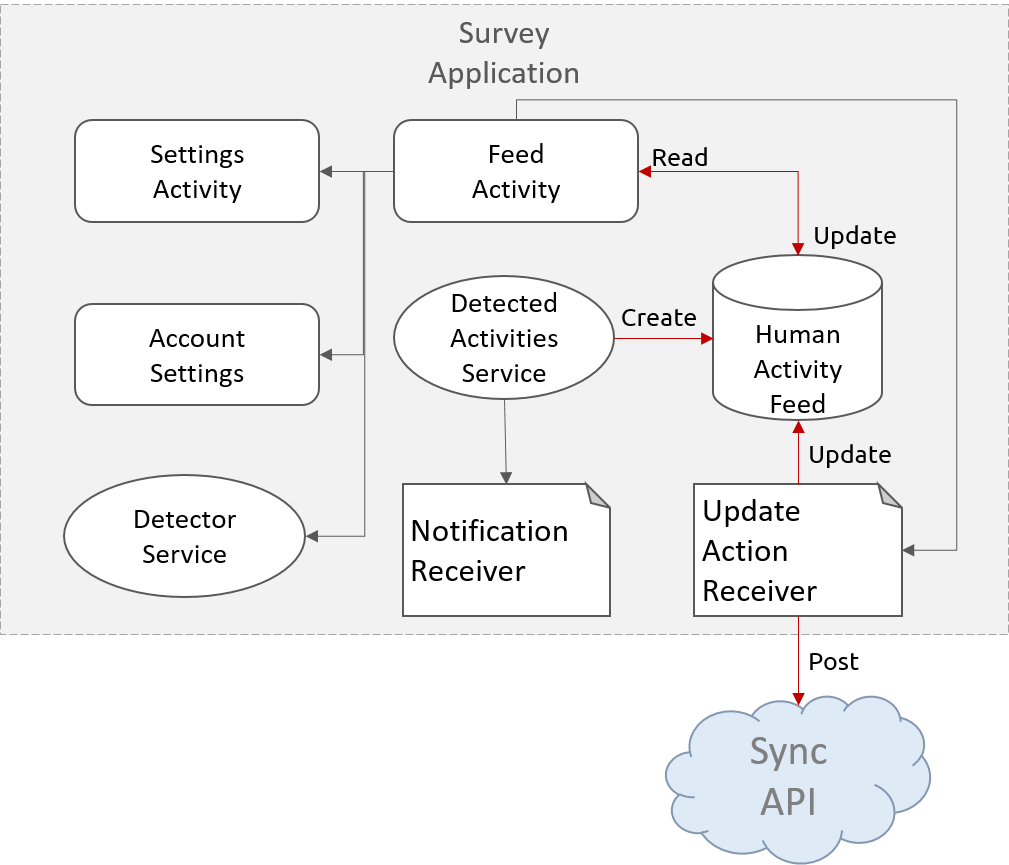
\includegraphics[width=0.65\columnwidth]{../capitulo-5/graphics/act_surv_diag}
\par\end{center}

\end{frame}
%
\begin{frame}{Backend C4.5: M�dulos Funcionales}

\setbeamercovered{transparent}
\begin{columns}

\column{0.5\textwidth}
\begin{itemize}
\item Servicio Web en \emph{Amazon AWS}
\item Base de datos 
\begin{itemize}
\item Conjunto entrenamiento inicial
\item Resultados de las encuestas
\end{itemize}
\item Modelo activo de aprendizaje por colaboraci�n
\end{itemize}

\column{0.5\textwidth}
\begin{center}
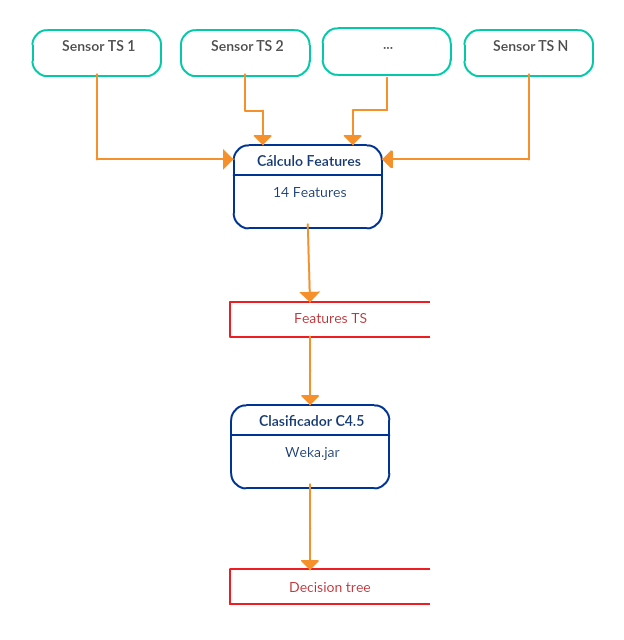
\includegraphics[height=1\linewidth]{../capitulo-6/graphics/proceso-genera-clasi}
\par\end{center}

\end{columns}

\end{frame}
%

